\secnumbersection{VALIDACIÓN DE LA SOLUCIÓN}
\label{sec:cap5}

La validación distingue el piloto del 5 de noviembre de 2024 del experimento mensual congelado. Este último agrega las 29 fechas disponibles entre el 1 y el 29 de noviembre, conserva tres inicializaciones por representación y libera la prueba una sola vez después de seleccionar los \textit{checkpoints} con validación. Las métricas se calculan con la definición de CPC de la ecuación~\eqref{eq:cpc_santiago}; la comparación sustantiva se realiza entre modelos que comparten soporte dentro de cada rama.

\subsection{Piloto como validación preliminar}
\label{sec:piloto_preliminar}

El piloto se realizó sobre el martes 5 de noviembre de 2024 para comprobar el recorrido de datos, el entrenamiento, la selección por validación y la evaluación sobre el soporte completo de destinos. Incluyó 15 corridas diagnósticas y nueve entrenamientos estables del día completo, con tres representaciones espaciales y tres inicializaciones por representación. Cada entrenamiento se limitó a 15 épocas. Las ventanas horarias tuvieron un propósito diagnóstico y no se usaron para establecer una comparación final entre períodos.

En la prueba del piloto, el CPC medio de Deep Gravity fue 0,4920 en Zona 777, 0,7172 en H3-r7 y 0,5623 en H3-r8. Las desviaciones estándar muestrales entre las tres inicializaciones fueron 0,0045, 0,0021 y 0,0017, respectivamente. Dentro de cada representación, el modelo de atracción entrenado obtuvo los CPC más altos, con 0,6457, 0,7764 y 0,6669. Estos resultados acreditan la factibilidad del procedimiento y muestran que la comparación con referencias debe conservarse en el experimento mensual; no acreditan convergencia, ajuste óptimo ni generalización temporal.

El experimento mensual no se interpreta como una réplica completamente independiente del piloto. Comparte la geografía de prueba y contiene el 5 de noviembre. La diferencia entre ambos escenarios reúne cambios de período, normalización, volumen de datos y presupuesto de entrenamiento, de modo que no puede atribuirse a un único factor.

\subsection{Soporte de prueba y caracterización espacial}
\label{sec:soporte_prueba}

El experimento principal agrega la cohorte final de 60.511.977 viajes, con masa expandida de 85.774.522,4070, observados entre el 1 y el 29 de noviembre de 2024. La Tabla~\ref{tab:soporte_prueba} hace explícitos los denominadores de prueba. Aunque la cohorte fuente es común, cada adaptador espacial asigna unidades, pares candidatos y masa de prueba propios. La evaluación mantiene el soporte completo de destinos para cada origen de prueba; las unidades sin origen asignado no se convierten en observaciones inactivas ni se eliminan del conjunto de destinos.

\begin{table}[htbp]
\centering
\scriptsize
\caption{Soporte de prueba por representación. Los pares positivos y su densidad se calculan sobre los pares candidatos indicados. La masa observada usa el factor de expansión; los orígenes activos e inactivos se refieren a la partición de prueba. Fuente: elaboración propia a partir de la tabla de soporte del experimento mensual.}
\label{tab:soporte_prueba}
\begin{tabular}{@{}lrrrrrr@{}}
\toprule
\textbf{Rama} & \textbf{Unid.} & \textbf{Orígenes} & \textbf{Sin asignar} & \textbf{Destinos} & \textbf{Pares candidatos} & \textbf{Masa exp.} \\
\midrule
Zona 777 & 793 & 101 (101/0) & 0 & 793 & 80.093 (61.132; 76,3\%) & 16,11 M \\
H3-r7 & 223 & 32 (32/0) & 5 & 223 & 7.136 (5.552; 77,8\%) & 17,39 M \\
H3-r8 & 1.210 & 189 (189/0) & 21 & 1.210 & 228.690 (99.374; 43,5\%) & 15,80 M \\
\bottomrule
\end{tabular}
\end{table}

En la columna de orígenes, el par entre paréntesis corresponde a activos/inactivos; en la columna de pares, el paréntesis contiene pares OD positivos y su densidad. La masa expandida se expresa en millones de unidades de masa observada. Los desgloses por origen y \textit{tile} se conservan como respaldo reproducible. La densidad de pares OD positivos fue 76,33\% en Zona 777, 77,80\% en H3-r7 y 43,45\% en H3-r8.

Las representaciones se construyen a partir de la misma cohorte, pero no comparten una partición de prueba idéntica una vez que cada viaje se asigna a una unidad espacial. Cambian el número de destinos por origen, los pares candidatos, la densidad OD y la masa de prueba. Por esta razón, el CPC no permite ordenar las tres representaciones como si fueran mediciones de una misma tarea. La comparación principal se realiza dentro de cada representación, contra referencias evaluadas en el mismo soporte.

La Figura~\ref{fig:concentracion_zona777} caracteriza la distribución espacial de la masa expandida en la rama zonal. Sus dos paneles usan la misma cohorte final y expresan concentración por superficie; no son mapas de error ni una medida de desempeño predictivo.

\begin{figure}[htbp]
\centering
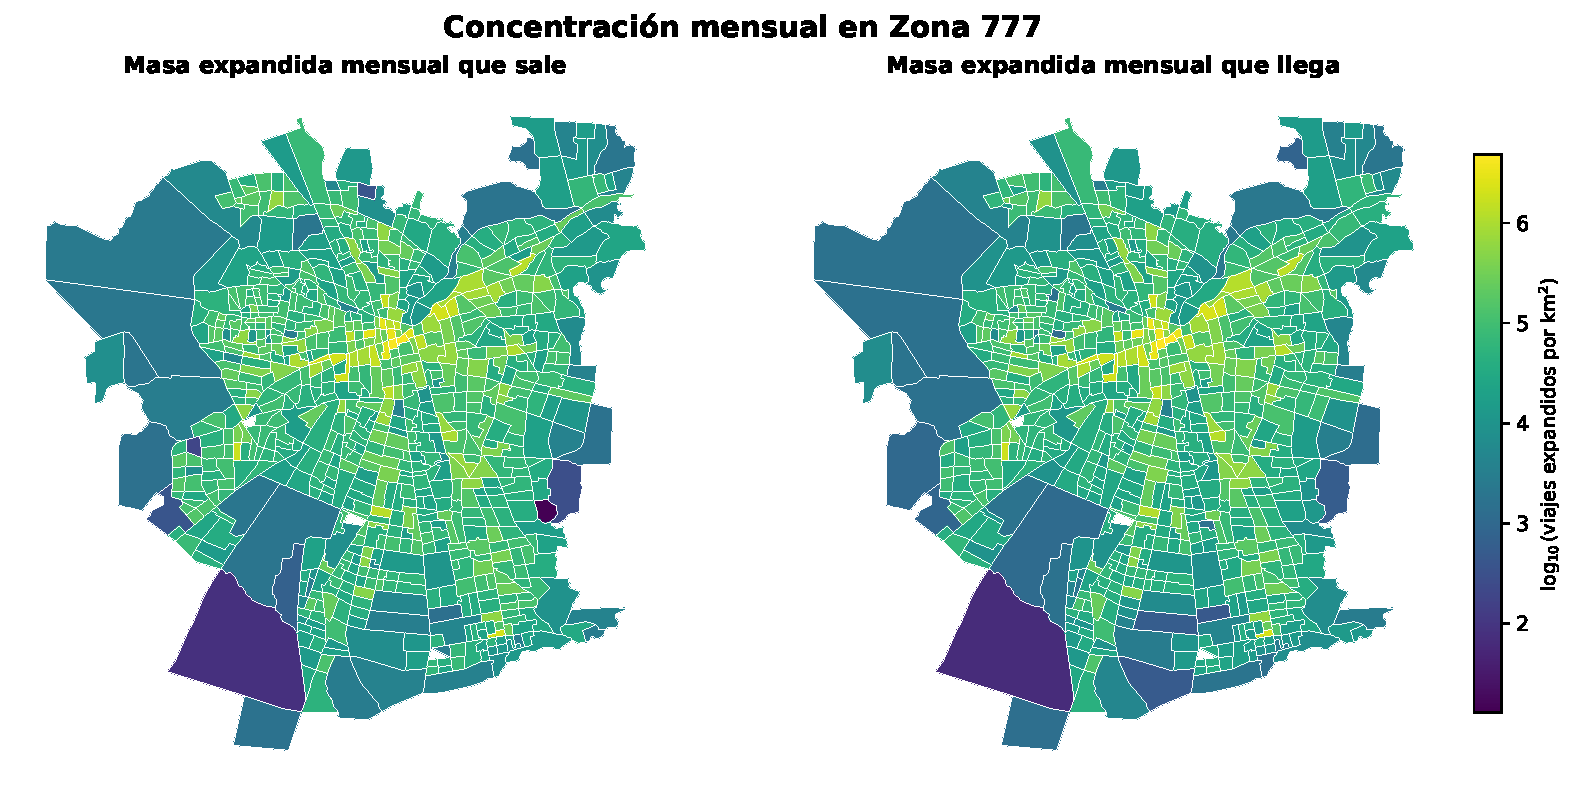
\includegraphics[width=\textwidth]{figures/v04_concentracion_origen_destino_zona777.pdf}
\caption{Concentración mensual de la masa expandida que sale y llega por km$^2$ en Zona 777. Cada panel usa la cohorte final de 60.511.977 viajes, del 1 al 29 de noviembre de 2024; los colores muestran $\log_{10}$ de masa expandida por km$^2$. Fuente: elaboración propia con datos DTPM y geometría oficial Zona 777.}
\label{fig:concentracion_zona777}
\end{figure}

\subsection{Resultados globales en prueba}
\label{sec:resultados_globales_prueba}

La Tabla~\ref{tab:resultados_prueba} reúne el CPC global de prueba con peso expandido. Deep Gravity se resume mediante media, desviación estándar muestral y rango de las tres inicializaciones; los modelos de referencia son deterministas y se ajustan solamente con los flujos de entrenamiento de la rama correspondiente. Las cifras no ordenan las representaciones entre sí, porque cambian las unidades, el soporte y la masa de prueba.

\begin{table}[htbp]
\centering
\scriptsize
\caption{CPC global de prueba con peso expandido y salida condicionada al flujo saliente observado. Deep Gravity se resume con tres inicializaciones independientes; DE es la desviación estándar muestral. Uniforme, atracción entrenada y gravedad exponencial se calculan una vez por rama sobre el mismo soporte de prueba. Fuente: elaboración propia a partir de los resultados mensuales congelados.}
\label{tab:resultados_prueba}
\begin{tabular}{@{}lccccc@{}}
\toprule
\textbf{Rama} & \textbf{Deep Gravity} & \textbf{Rango} & \textbf{Uniforme} & \textbf{Atracción} & \textbf{Gravedad exp.} \\
\midrule
Zona 777 & 0,5609 $\pm$ 0,0062 & 0,5537--0,5647 & 0,2992 & 0,6574 & 0,3819 \\
H3-r7 & 0,7722 $\pm$ 0,0060 & 0,7671--0,7787 & 0,3702 & 0,7757 & 0,6153 \\
H3-r8 & 0,6079 $\pm$ 0,0047 & 0,6046--0,6133 & 0,2611 & 0,6867 & 0,3777 \\
\bottomrule
\end{tabular}
\end{table}

La Figura~\ref{fig:cpc_semillas_referencias} muestra los mismos resultados sin ocultar las tres semillas. Los cuadrados corresponden a los modelos de referencia y los círculos a inicializaciones de Deep Gravity; la lectura válida sigue siendo dentro de cada panel o rama.

\begin{figure}[htbp]
\centering
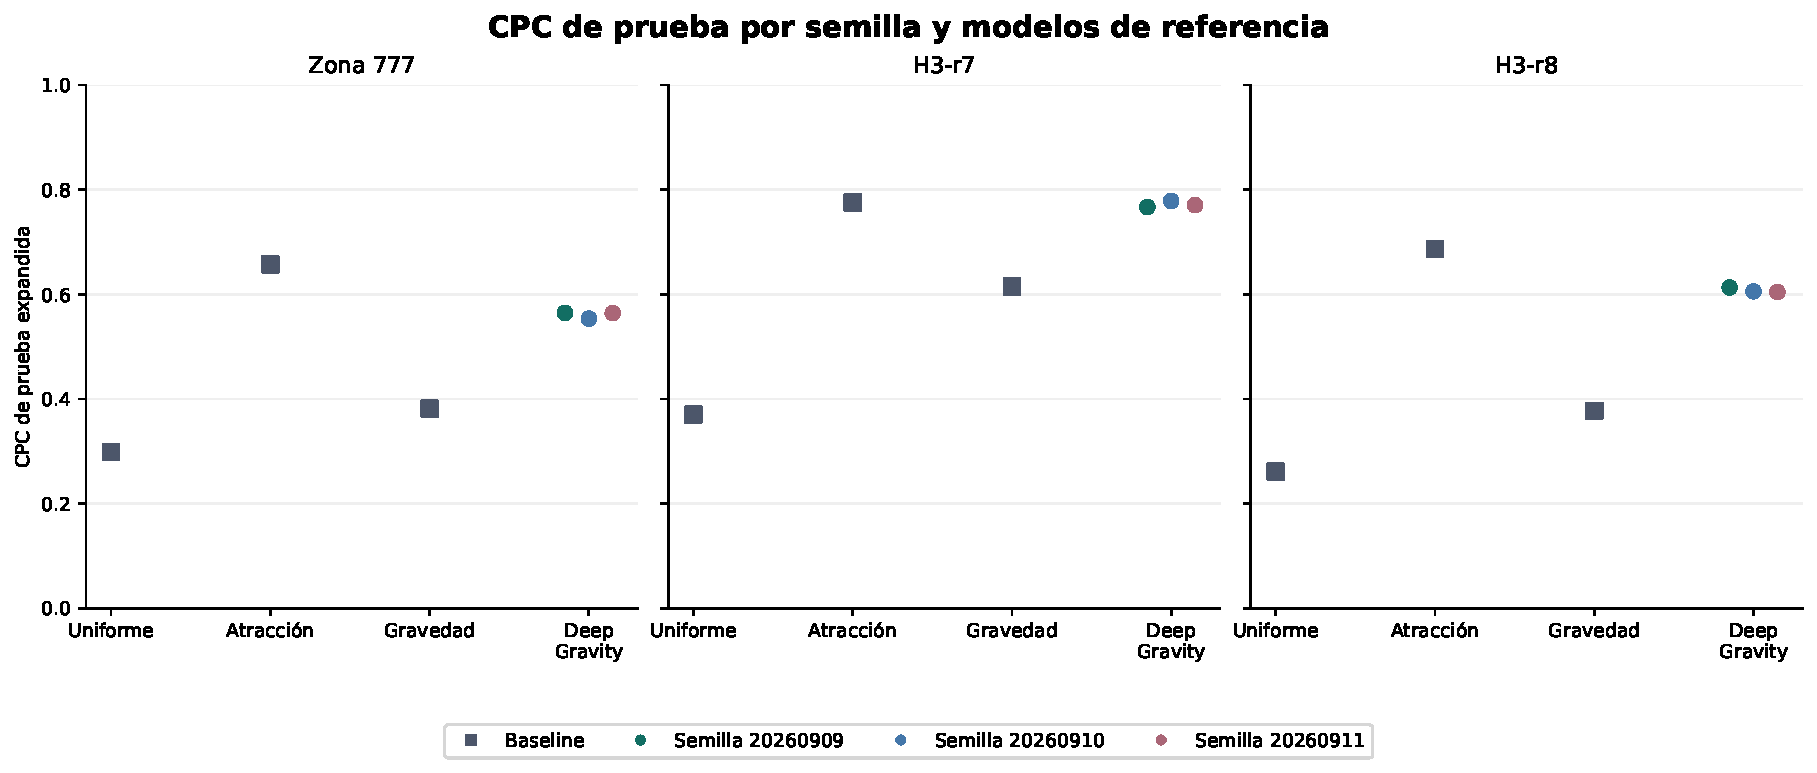
\includegraphics[width=\textwidth]{figures/cpc_semillas_y_referencias.pdf}
\caption{CPC de prueba expandida por semilla y modelos de referencia. Cada panel corresponde a una representación y mantiene su propio soporte de destinos; los cuadrados son referencias deterministas y los círculos son las semillas 20260909, 20260910 y 20260911 de Deep Gravity. Fuente: elaboración propia a partir de las métricas globales del experimento mensual.}
\label{fig:cpc_semillas_referencias}
\end{figure}

Deep Gravity superó las referencias uniforme y de gravedad exponencial en las tres representaciones. En Zona 777, el CPC medio fue 0,5609, frente a 0,2992 para la referencia uniforme y 0,3819 para la referencia gravitacional. En H3-r7, los valores fueron 0,7722, 0,3702 y 0,6153. En H3-r8, fueron 0,6079, 0,2611 y 0,3777. La magnitud de esas diferencias sólo se interpreta dentro de cada representación porque el soporte y la agregación cambian entre ellas.

La referencia de atracción entrenada superó la media de Deep Gravity en las tres representaciones: 0,6574 frente a 0,5609 en Zona 777, 0,7757 frente a 0,7722 en H3-r7 y 0,6867 frente a 0,6079 en H3-r8. La diferencia fue particularmente pequeña en H3-r7, donde una inicialización de Deep Gravity alcanzó 0,7787 y superó individualmente el valor de atracción. Esa observación no altera el resumen de las tres inicializaciones ni autoriza seleccionar una semilla a partir de prueba. El resultado principal es que, bajo esta configuración, la red mejora sobre las referencias uniforme y gravitacional, pero no supera en promedio a la referencia de atracción ajustada con entrenamiento.

La conservación de masa se verificó para todos los orígenes de prueba. El mayor error absoluto por origen fue $1{,}863\times10^{-9}$. Este control confirma que la conversión de probabilidades en flujos preserva el flujo saliente observado, sin convertir la tarea en un modelo de generación total de viajes.

\subsection{Trayectorias y selección por validación}
\label{sec:trayectorias_validacion}

La Figura~\ref{fig:trayectorias_mensuales} conserva las trayectorias de las nueve corridas y permite distinguir la pérdida de entrenamiento del CPC de validación utilizado para elegir los \textit{checkpoints}. La línea vertical discontinua marca el límite inicial de 200 épocas; solo Zona 777--20260909 y H3-r8--20260910 continuaron mediante las extensiones autorizadas, sin alterar datos, arquitectura, optimizador, particiones o regla de selección.

\begin{figure}[htbp]
\centering
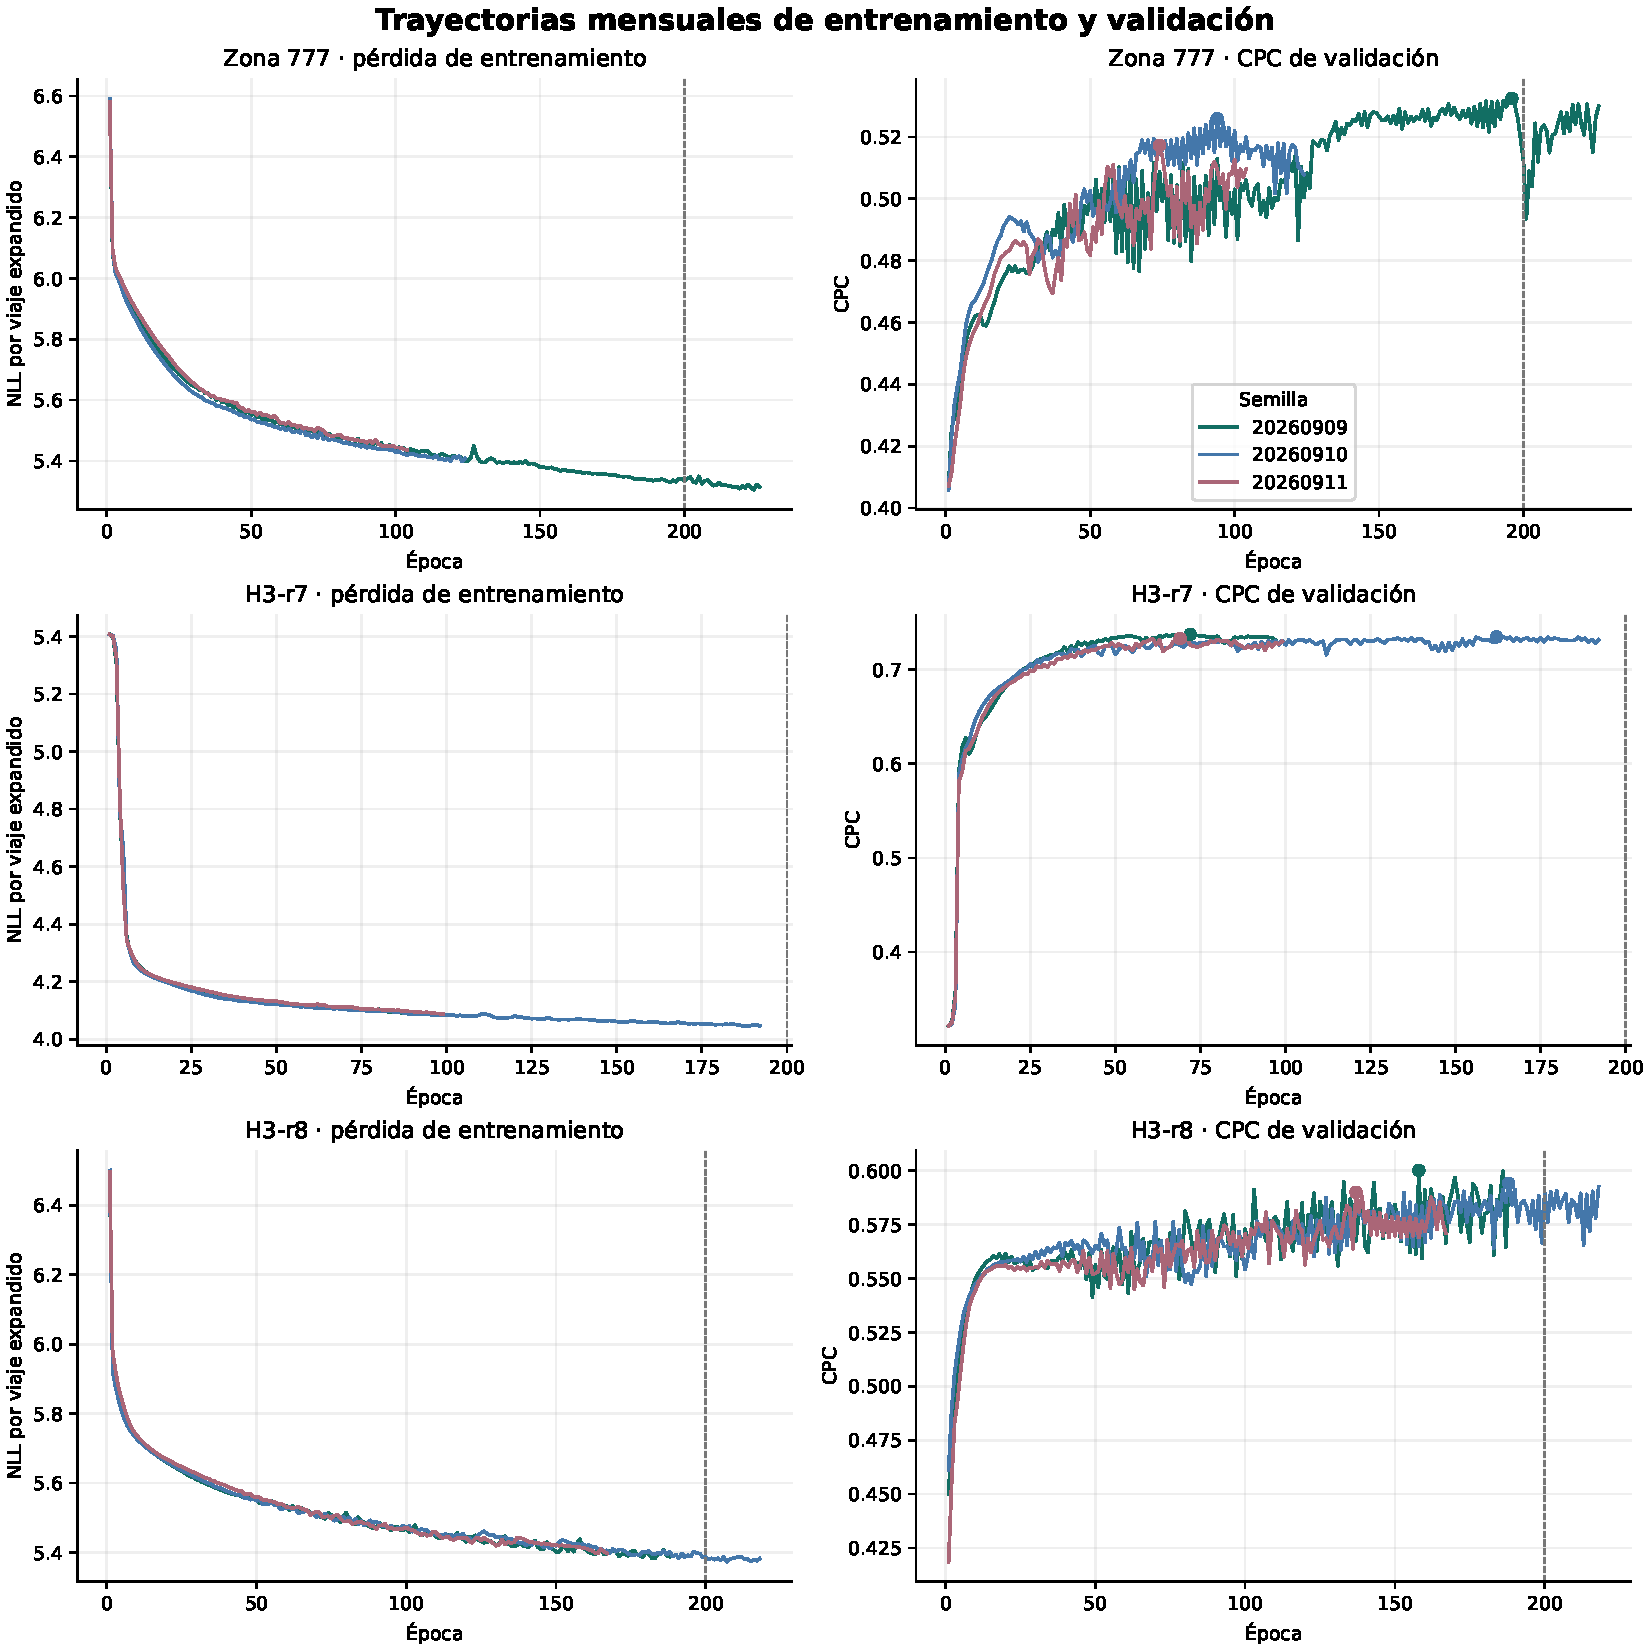
\includegraphics[width=0.88\textwidth]{figures/trayectorias_entrenamiento_validacion.pdf}
\caption{Trayectorias mensuales de pérdida de entrenamiento y CPC global de validación para las tres semillas de cada rama. La pérdida se expresa como NLL por viaje expandido; los puntos destacados marcan los \textit{checkpoints} seleccionados por CPC de validación y la línea discontinua señala la época 200. Fuente: elaboración propia a partir de las trayectorias del experimento mensual.}
\label{fig:trayectorias_mensuales}
\end{figure}

Todas las corridas cerraron por meseta de validación. Las dos extensiones no alteraron datos, particiones, arquitectura, optimizador ni regla de selección. La corrida de Zona 777 con semilla 20260909 cerró en la época 226 y mantuvo como \textit{checkpoint} seleccionado la época 196. La corrida de H3-r8 con semilla 20260910 cerró en la época 218 y mantuvo la época 188. Las restantes siete corridas cerraron sin extensión.

Los rangos de CPC de prueba entre las tres inicializaciones fueron 0,0110 en Zona 777, 0,0117 en H3-r7 y 0,0087 en H3-r8. Ninguno excedió la alerta protocolaria de 0,05. Esta dispersión describe la variación asociada a la inicialización y al entrenamiento bajo una partición espacial fija. No estima incertidumbre poblacional, variación entre particiones ni significación estadística.

Una verificación independiente volvió a evaluar un \textit{checkpoint} seleccionado por validación en cada representación. Las diferencias absolutas de CPC fueron inferiores a $10^{-6}$, con soporte completo de destinos. Esta comprobación respalda la consistencia técnica de la evaluación congelada, pero no equivale a una validación científica en otra ciudad, período o partición espacial.

\subsection{Sensibilidad al peso de evaluación}
\label{sec:sensibilidad_peso}

La Figura~\ref{fig:sensibilidad_pesos} contrasta el CPC calculado con masa expandida y con conteos sin expansión. En ambos ejes se aplican las mismas probabilidades ya congeladas y cada origen se reescala con su respectivo flujo saliente; el eje sin expansión no corresponde a un reentrenamiento ni a una nueva selección de modelos. La diagonal indica igualdad entre ambas evaluaciones.

\begin{figure}[htbp]
\centering
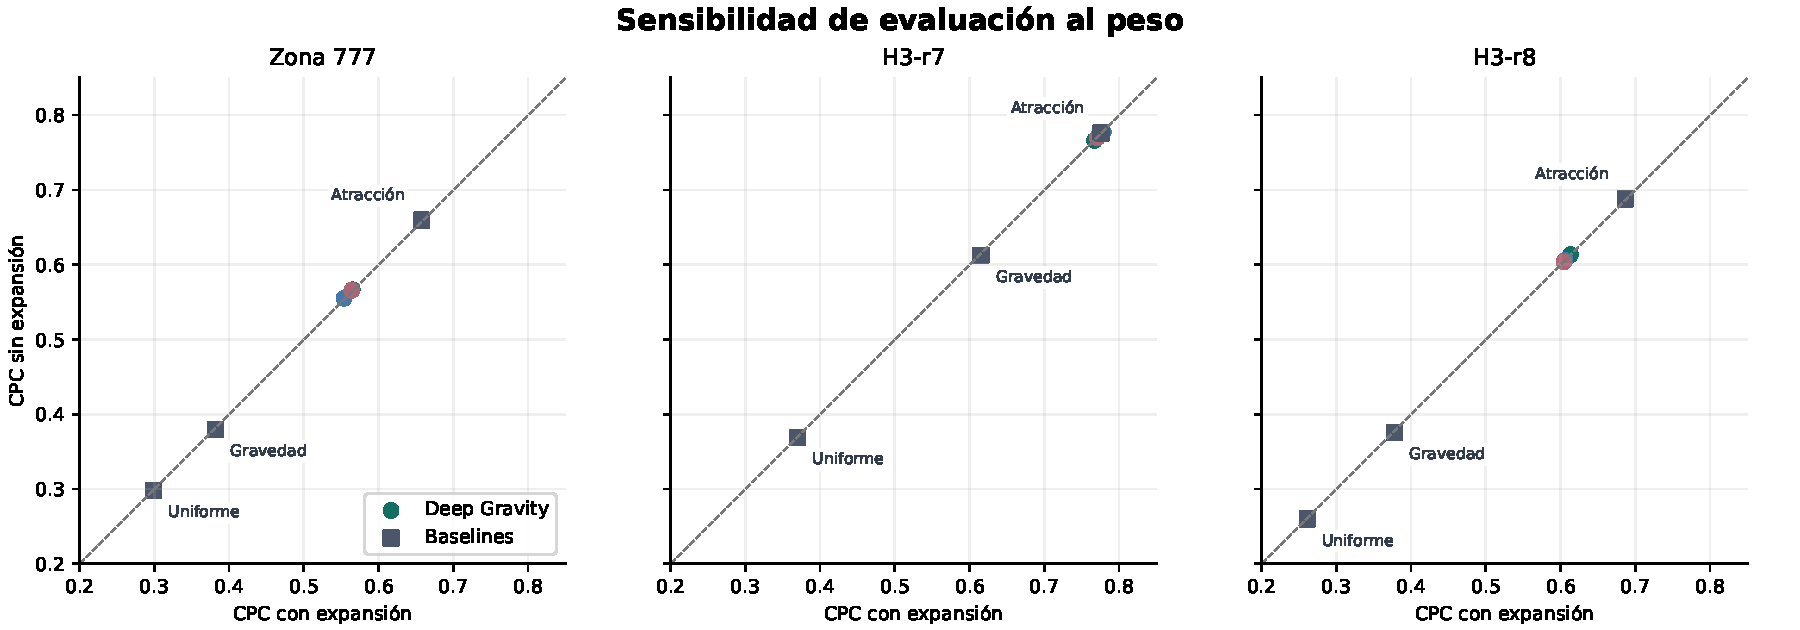
\includegraphics[width=\textwidth]{figures/sensibilidad_pesos.pdf}
\caption{Sensibilidad del CPC de prueba al peso de evaluación. El eje horizontal usa masa expandida y el vertical conteos OD sin expansión; los círculos corresponden a las tres semillas de Deep Gravity y los cuadrados a los modelos de referencia. Cada punto reutiliza probabilidades congeladas y conserva los parámetros de las referencias ajustadas con peso expandido. La diagonal discontinua representa igualdad entre ambas métricas. Fuente: elaboración propia a partir de la evaluación de sensibilidad mensual.}
\label{fig:sensibilidad_pesos}
\end{figure}

El cambio de ponderación no modificó la lectura comparativa principal. Los CPC medios de Deep Gravity fueron 0,5623 en Zona 777, 0,7711 en H3-r7 y 0,6077 en H3-r8 al usar conteos sin expansión, frente a 0,5609, 0,7722 y 0,6079 con masa expandida. La atracción entrenada siguió sobre la media de la red en las tres representaciones. La figura debe leerse como una sensibilidad de evaluación al uso del peso, no como evidencia de que los modelos tendrían el mismo comportamiento después de reentrenarse con otra función de pérdida.

\subsection{Recursos de ejecución}
\label{sec:recursos_ejecucion}

La Tabla~\ref{tab:costos_ejecucion} registra los recursos observados durante las épocas de entrenamiento y validación. Estos tiempos excluyen carga inicial y escritura de \textit{checkpoints}, por lo que el total es una cota inferior del costo operativo y no un presupuesto integral de ejecución.

\begin{table}[htbp]
\centering
\small
\caption{Recursos observados para las nueve corridas mensuales. Las horas corresponden a entrenamiento y validación; la memoria es el máximo registrado en las corridas de cada fila; el tamaño de artefactos se convierte de bytes a GiB ($2^{30}$ bytes) y se redondea a dos decimales. Fuente: elaboración propia a partir del registro de costos e incidencias del experimento mensual.}
\label{tab:costos_ejecucion}
\begin{tabular}{@{}lrrrr@{}}
\toprule
\textbf{Rama} & \textbf{Corridas} & \textbf{Horas} & \textbf{Memoria máx. (GiB)} & \textbf{Artefactos (GiB)} \\
\midrule
Zona 777 & 3 & 2,62 & 0,53 & 2,33 \\
H3-r7 & 3 & 0,19 & 0,53 & 1,99 \\
H3-r8 & 3 & 6,65 & 0,83 & 2,95 \\
\midrule
Total de nueve corridas & 9 & 9,46 & 0,83 & 7,27 \\
\bottomrule
\end{tabular}
\end{table}

Las nueve corridas acumularon 9,46 horas de entrenamiento y validación. El desglose fue 0,19 horas en H3-r7, 2,62 horas en Zona 777 y 6,65 horas en H3-r8. El máximo de memoria de proceso observado fue 0,834 GiB. Estas cifras describen los recursos medidos, no el costo operativo completo.

Se registraron dos incidencias sin efecto sobre los resultados de prueba. Antes de la primera época, una corrida de Zona 777 no resolvía un parámetro de hilos de CPU; la corrección se aplicó antes de producir entrenamiento o prueba y no se contabilizó como una inicialización adicional. Más tarde, un primer intento de verificación no pudo serializar una ruta relativa después de crear archivos parciales de reproducción. La verificación final se ejecutó en un directorio nuevo y los archivos parciales quedaron fuera de la evidencia. Ninguna incidencia modificó \textit{checkpoints}, resultados congelados ni la liberación de prueba.

Los desgloses por corrida, origen y \textit{tile}, junto con las verificaciones de conservación de masa y los replays técnicos, permanecen en el respaldo reproducible.

\subsection{Resultado del análisis complementario de atribuciones predictivas}
\label{sec:resultado_xai}

El análisis complementario evaluó tres aproximaciones para atribuir cambios en la log-probabilidad condicional de un destino dentro del soporte completo de cada origen. Las explicaciones se definieron como sensibilidades predictivas dependientes de la salida, de la muestra y de las referencias de entrenamiento. No se interpretaron como efectos causales.

La primera aproximación, basada en gradientes integrados, no acreditó completitud para una consulta crítica aun al aumentar la cuadratura hasta 4.096 nodos. La segunda, basada en permutaciones agrupadas, no acreditó la estabilidad entre dos conjuntos independientes de fondos en dos de las tres inicializaciones de la primera consulta obligatoria. La tercera, basada en valores de Shapley exactos para grupos jerárquicos, acreditó una primera consulta con 24 fondos por conjunto, pero una segunda consulta crítica no alcanzó la estabilidad requerida de los tres supergrupos con 24 ni con 48 fondos.

Ninguna aproximación superó todos los controles definidos antes de la ejecución. Por ello, no se publican rankings, atribuciones, figuras SHAP ni casos locales. El resultado es metodológico: bajo las configuraciones evaluadas no se obtuvieron atribuciones suficientemente estables para una interpretación sustantiva de las características territoriales. Este desenlace limita la interpretabilidad disponible, pero no modifica las métricas predictivas ni las comparaciones con referencias, que se obtuvieron con un protocolo de evaluación distinto.

\subsection{Discusión y amenazas a la validez}
\label{sec:discusion_amenazas_validez}

La evaluación muestra que Deep Gravity puede ejecutarse de forma trazable sobre la cohorte DTPM y producir una distribución de destinos que supera las referencias uniforme y de gravedad exponencial en las tres representaciones examinadas. Sin embargo, la referencia de atracción entrenada obtiene un CPC medio mayor en las tres ramas. Este resultado evita presentar la red como una mejora general sobre todas las referencias y concentra la interpretación en las condiciones concretas de la evaluación.

La reproducción técnica previa del código con datos de Nueva York se conserva como antecedente de compatibilidad de implementación. No reproduce el contexto empírico de Santiago ni funciona como un control equivalente, por lo que sus métricas no se comparan con los CPC de este capítulo.

La discretización espacial modifica el problema evaluado. H3-r7, H3-r8 y Zona 777 no sólo difieren en tamaño o forma de unidad: cambian los destinos disponibles, la densidad de pares OD positivos, la masa de prueba y la agregación de atributos. La sensibilidad observada entre representaciones es informativa para describir ese efecto de agregación, pero no permite declarar una resolución ganadora a partir del CPC global.

La validez temporal queda acotada a las 29 fechas disponibles de noviembre de 2024. La validez espacial queda acotada a una sola partición de origen, concentrada en un \textit{tile} de prueba, y a las 34 comunas del dominio definido. El piloto comparte la geografía de prueba y una de las fechas del agregado mensual. En consecuencia, los resultados no constituyen una validación temporal ni espacial independiente del piloto.

La fuente DTPM representa viajes reconstruibles de transporte público y no toda la movilidad urbana. La distribución predicha está condicionada al flujo saliente observado, por lo que no estima la generación de viajes por origen. Además, la cobertura de OpenStreetMap corresponde a una instantánea anterior a los viajes y la interpolación del Censo 2024 supone distribución uniforme dentro de cada geometría censal. Las decisiones de reconstrucción de viajes, exclusión de zonas sin polígono y asignación a unidades espaciales también condicionan el resultado.

Las tres inicializaciones permiten describir variación de entrenamiento, pero no reemplazan particiones espaciales adicionales ni una muestra poblacional de experimentos. El resultado no validado del análisis de atribuciones añade una limitación específica: los resultados predictivos no pueden acompañarse de una explicación estable de la contribución de cada atributo bajo las configuraciones ensayadas. Una extensión futura debería separar explícitamente la validación temporal y espacial, incorporar particiones adicionales y definir un protocolo explicativo con controles que pueda acreditar estabilidad antes de interpretar atribuciones.

